\documentclass[12pt,oneside,a4paper,english]{article}
\usepackage[T1]{fontenc}
\usepackage[latin2]{inputenc}
\usepackage[margin=2.25cm,headheight=26pt,includeheadfoot]{geometry}
\usepackage[english]{babel}
\usepackage{listings}
\usepackage{color}
\usepackage{titlesec}
\usepackage{titling}
\usepackage[framed, numbered]{matlab-prettifier}
\usepackage{changepage}
\usepackage{amsmath}
\usepackage{hyperref}
\usepackage{enumitem}
\usepackage{graphicx}
\usepackage{fancyhdr}
\usepackage{lastpage}
\usepackage{caption}
\usepackage{tocloft}
\usepackage{setspace}
\usepackage{multirow}
\usepackage{titling}
\usepackage{float}
\usepackage{comment}
\usepackage{booktabs}
\usepackage{indentfirst}
\usepackage{lscape}
\usepackage{booktabs,caption}
\usepackage[flushleft]{threeparttable}
\usepackage[english]{nomencl}
\usepackage{xcolor}
\usepackage{lipsum}


% --- set footer and header ---
\pagestyle{fancy}
\fancyhf{}

\setlength{\parindent}{2em}
\title{Introduction to Alderbaran Characteristics and Spectrum} % to reference as \title, dont use \maketitle
\makeatletter\let\Title\@title\makeatother



\lstset{language=Matlab,
style=Matlab-editor,
basicstyle=\normalsize\mlttfamily,
numbers=left,
numberstyle={\scriptsize\color{black}},			% size of the numbers
numbersep=0.5cm											
}

\newlist{steps}{enumerate}{1}
\setlist[steps, 1]{leftmargin=1.5cm,label = Step \arabic*:}
\renewcommand{\headrulewidth}{1pt}
\renewcommand{\footrulewidth}{1pt}

%\lhead{\Title}
\rhead{\nouppercase{\rightmark}}
\lhead{\Title}
\rfoot{
\includegraphics[height=1.25cm]{root/logo.pdf}} % right header logo
\setlength\headheight{16pt}
\setlength{\footskip}{50pt}
\lhead{\Title} %rightH title
\cfoot{\thepage}

% --- End of page settings ---



\begin{document}
\pagenumbering{roman} 

\begin{titlepage}
\begin{center}
\vspace{2cm}
%\textsc{ Danmarks Tekniske Universitet}\\[1.5cm]
\vspace{2cm}

\vspace{2cm}

% Title
\hrule
\vspace{.5cm}
{ \huge \bfseries Introduction to Alderbaran Characteristics and Spectrum} % title of the report
\vspace{.5cm}

\hrule
\vspace{1.5cm}

\textsc{\textbf{Authors}}\\
\vspace{.5cm}
\centering

% add your name here
Zachary Shelton 
\vspace{4cm}

\centering \today % Dags dato
\end{center}
\end{titlepage}
\doublespacing
%\addcontentsline{toc}{section}{Table of Contents}
\renewcommand{\baselinestretch}{1}\normalsize
\tableofcontents
\renewcommand{\baselinestretch}{1}\normalsize
%\singlespacing
\thispagestyle{fancy} % force page style
\newpage
\section{Abstract}
There are billions of stars and celestial bodies that are worthwhile for scientist and astronomers to observe. When focusing on one body, it requires navigating various databases and academic journals to find characteristics of the body. This paper will focus on the star Alderbaran, which is the brightest star in the constellation Taurus. The paper will discuss the characteristics of Alderbaran, including its class, mass, and temperature. It will also outline how to find the same information for other celestial bodies. 

\section{Celestial Databases}
There is so much observational data it feels impossible to find a specific piece of data or information. However, there are tools and databases that can help. The first tool is the \href{https://cds.unistra.fr/}{SIMBAD database}, which is a database of astronomical objects. The database provides basic information about celestial bodies, such as their class, mass, and temperature. There is also second tool is the \href{https://vizier.cds.unistra.fr/viz-bin/VizieR}{VizieR database}, which provides detailed information about similar or same celestial bodies, such as their spectral type, luminosity, and radius. If your interested in exoplanets, there is the Exoplanet Archive, which provides information about observed and theorized exoplanets, such as their mass, radius, and orbital period.

\section{Glossary of Important Terms}
This section will cover a not so comprehensive list of terms used in astronomy and their meanings:
\begin{itemize}
    \item \textbf{Stellar Class} - The class of a star is a letter that represents the temperature of the star. The classes are O, B, A, F, G, K, and M. The O class is the hottest and the M class is the coolest. These correspond to the mass and temperature of the star,  \textbf{Sometimes called spectral type.}
    \item  \textbf{Blackbody Radiation} - Blackbody radiation is the radiation that is emitted by a blackbody(read more at: \href{https://phys.libretexts.org/Bookshelves/University_Physics/University_Physics_(OpenStax)/University_Physics_III_-_Optics_and_Modern_Physics_(OpenStax)/06%3A_Photons_and_Matter_Waves/6.02%3A_Blackbody_Radiation}{Blackbody Radiation}). By measuring the broad spectrum of wavelengths of stars, scientist to can determine the temperature of the star.
    \item \textbf{Wien's Law} - States the peak wavelength of a blackbody is inversely proportional to the temperature of the blackbody. The law is represented by the equation $\lambda_{\text{max}} = \frac{b}{T}$, where $\lambda_{\text{max}}$ is the peak wavelength, $b=2.89*10^{-3} m \cdot K$ is Wien's constant, and $T$ is the temperature of the blackbody.
    \item \textbf{Stellar Mass} - Astronomers and astorphysicist use the spectrum of the star combined with the star's luminosity to determine the mass of the star. The peak wavelength of a star indicates what a star is made of. This mass is given generally in solar masses, proportional to the mass of the sun.
    \item \textbf{Stellar Luminosity} - A measure of the total energy a celestial body releases each second, this is also know as absolute brigtness. There are many ways to measure this, and there are definite challenges in determining the true brightness of any stellar body far away.(Read More at: \href{https://www.teachastronomy.com/textbook/Properties-of-Stars/Stellar-Luminosity/}{Stellar Luminosity})
\end{itemize}

\section{Learning About Alderbaran}
Heading to \href{https://simbad.cds.unistra.fr/simbad/}{SINBAD}, we can search for Alderbaran and find general characteristics of the star. Alderbaran is an indentifier, however there are many more celestial bodies to give each a unique name, so the identifier is a combination of numbers and letters. The identifier for Alderbaran is HIP 21421 or Alpha Tauri.
\begin{figure}[H]
    \centering
    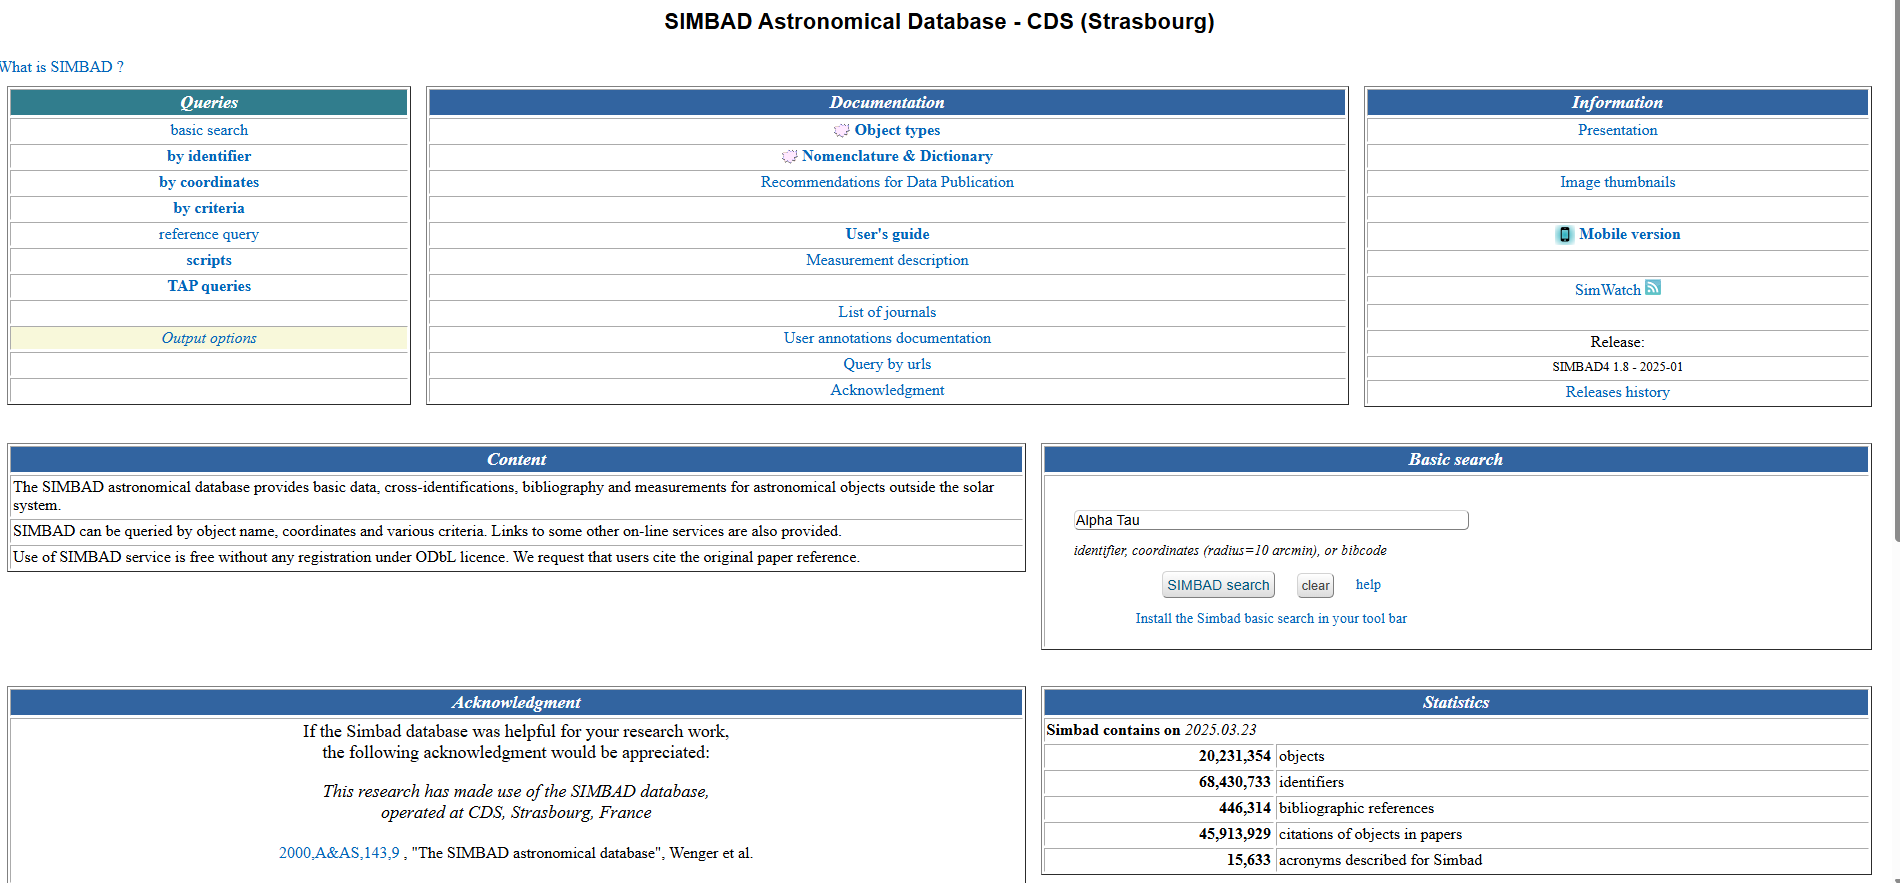
\includegraphics[width=0.75\textwidth]{SINBAD1.png}
    \caption{SIMBAD Database homepage, search for Alderbaran using one of its identifier}
\end{figure}
Completing the search will take you directly to the star Alderbaran. The page will show the star's class, mass, and temperature. The class of Alderbaran is K5III, which means it is a cool star. 
\begin{figure}
    \centering
    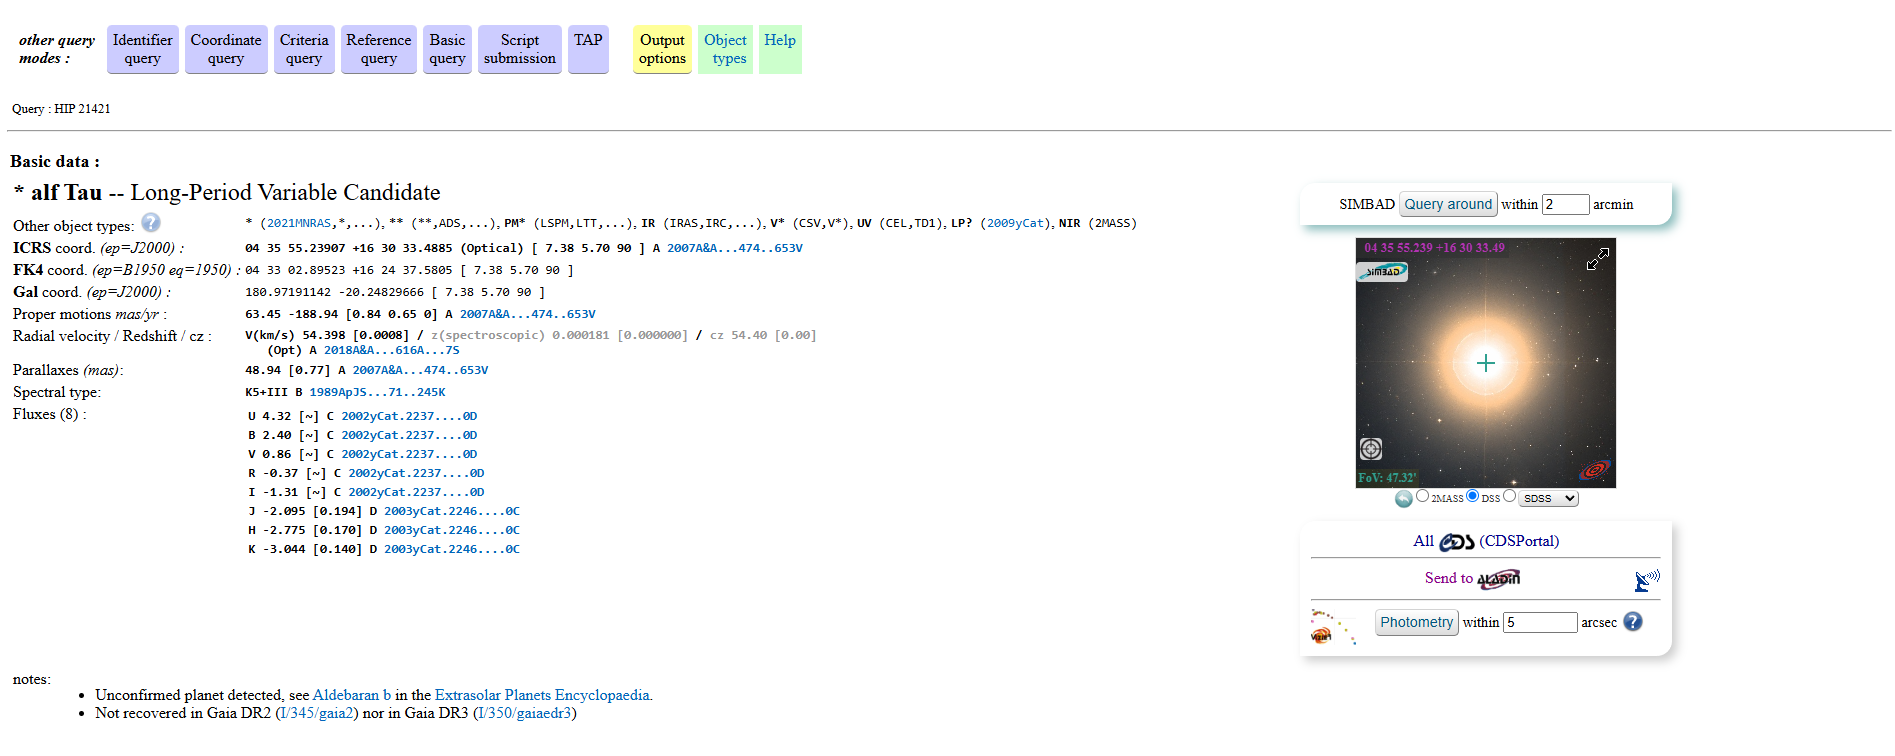
\includegraphics[width=0.75\textwidth]{SINBAD2.png}
    \caption{SIMBAD Database page for Alderbaran, note the class, mass, and temperature of the star}
\end{figure}

\label{endOfDoc}
\end{document}
